%------------------------------------------------------------------------------------------------%

\chapter{Running the Solver xspecfem2D}

%------------------------------------------------------------------------------------------------%

To run the solver, type
%
\begin{verbatim}
    bin/xspecfem2D
\end{verbatim}
%
from within the main working directory (use \texttt{mpirun} or equivalent if you compiled with parallel support). This will output the seismograms and snapshots of the wave fronts at different time steps in directory \texttt{OUTPUT\_FILES/}. To visualize them, type "\texttt{gs OUTPUT\_FILES/vect*.ps}" to see the Postscript files (in which the wave field is represented with small arrows, fluid/solid matching interfaces with a thick pink line, and absorbing edges with a thick green line) and "\texttt{gimp OUTPUT\_FILES/image*.gif}" to see the colour snapshot showing a pixelized image of one of the two components of the wave field (or pressure, depending on what you have selected for the output in \texttt{DATA/Par\_file}).

%%
\begin{figure}[htbp]
\centering
\includegraphics[width=2in]{figures/image0000300.jpg}
\includegraphics[width=2in]{figures/image0000400.jpg}
\includegraphics[width=2in]{figures/image0000500.jpg}
\caption{Wavefield snapshots of the default example generated by \texttt{xspecfem2D} when parameter \texttt{output\_color\_image} is set to \texttt{.true.}. To create smaller (subsampled) images you can change double precision parameter \texttt{factor\_subsample\_image = 1.0} to a higher value in file \texttt{DATA/Par\_file}. This can be useful in the case of very large models. The number of pixels of the image in each direction must be smaller than parameter \texttt{NX\_NZ\_IMAGE\_MAX} defined in file \texttt{SETUP/constants.h.in}, again to avoid creating huge images in the case of very large models.}
\label{fig:example.solver}
\end{figure}
%%

Please consider these following points, when running the solver:
%
\begin{itemize}
\item the \texttt{DATA/Par\_file} given with the code works fine, you can use it without any modification to test the code

\item the seismograms \texttt{OUTPUT\_FILES/*.sem*} are simple ASCII files with two columns: time in the first column and amplitude in the second, therefore they can be visualized with any tool you like, for instance ``\texttt{gnuplot}''; if you prefer to output binary seismograms in Seismic Unix format (which is a simple binary array dump) you can use parameter \texttt{SU\_FORMAT}, in which case all the seismograms will be written to a single file with the extension \texttt{*.bin}.
Depending on your installation of the Seismic Unix package you can use one of these two commands:
%
\begin{verbatim}
    surange < Uz_file_single.bin
    suoldtonew < Uz_file_single.bin | surange
\end{verbatim}
%
to see the header info.
Replace \texttt{surange} with \texttt{suxwigb} to see wiggle plots for the seismograms.

\item if flag \texttt{MODEL} in \texttt{DATA/Par\_file} is set to \texttt{default}, the velocity and density model is determined using the \texttt{nbmodels} and \texttt{nbregions} devices.  Otherwise, \texttt{nbmodels} values are ignored and the velocity and density model is determined from a user supplied file or subroutine.

\item when compiling with Intel ifort, use ``\texttt{-assume byterecl}'' option to create binary PNM images displaying the wave field

\item there are a few useful scripts and Fortran routines in directory \texttt{utils/}.

\item you can find a Fortran code to compute the analytical solution for simple media that we use as a reference in benchmarks in many of our articles at
\urlwithparentheses{http://www.spice-rtn.org/library/software/EX2DDIR}. That code is described in: \cite{BeIfNiSk94}

\end{itemize}

%------------------------------------------------------------------------------------------------%
\section*{Notes about \texttt{DATA/Par\_file} parameters}
%------------------------------------------------------------------------------------------------%

The default \texttt{DATA/Par\_file} provided in the root directory of the code contains detailed comments and should be almost self-explanatory
(note that some of the older \texttt{DATA/Par\_file} files provided in the \texttt{EXAMPLES} directory work fine but some of the comments
they contain may be obsolete or even wrong; thus refer to the default \texttt{DATA/Par\_file} instead for reliable explanations).

\begin{description}[font=\ttfamily]

\item[USE\_TRICK\_FOR\_BETTER\_PRESSURE]

This option can only be used so far if all the receivers record pressure and are in acoustic elements.
Use a trick to increase accuracy of pressure seismograms in fluid (acoustic) elements:
use the second derivative of the source for the source time function instead of the source itself,
and then record \texttt{potential\_acoustic()} as pressure seismograms instead of \texttt{potential\_dot\_dot\_acoustic()};
this is mathematically equivalent, but numerically significantly more accurate because in the explicit
Newmark time scheme acceleration is accurate at zeroth order while displacement is accurate at second order,
thus in fluid elements \texttt{potential\_dot\_dot\_acoustic()} is accurate at zeroth order while \texttt{potential\_acoustic()}
is accurate at second order and thus contains significantly less numerical noise.

%use a trick to increase accuracy of pressure seismograms in fluid (acoustic) elements: use the second derivative of the source for the source time function instead of the source itself, and then record -potential\_acoustic() as pressure seismograms instead of -potential\_dot\_dot_acoustic(); this is mathematically equivalent, but numerically significantly more accurate because in the explicit Newmark time scheme acceleration is accurate at zeroth order while displacement is accurate at second order, thus in fluid elements potential\_dot\_dot_acoustic() is accurate at zeroth order while potential\_acoustic() is accurate at second order and thus contains significantly less numerical noise.


\item[READ\_VELOCITIES\_AT\_f0]

 shift (i.e. change) velocities read from the input file to take average physical dispersion into account, i.e. if needed change the reference frequency at which these velocities are defined internally in the code: by default, the velocity values that are read at the end of this Par\_file of the code are supposed to be the unrelaxed values, i.e. the velocities at infinite frequency. If you set this flage to .true., the values read are then those for a given frequency called ATTENUATION\_f0\_REFERENCE.


\item[nbmodels]  With \texttt{MODEL = default} chosen, a variety of simple velocity and density models can be defined using the \texttt{nbmodels} device.

%
\begin{verbatim}
I:  model_number 1 rho Vp Vs 0 0 QKappa Qmu 0 0 0 0 0 0
II:  model_number 2 rho c11 c13 c15 c33 c35 c55 c12 c23 c25 0 QKappa Qmu
III: model_number 3 rhos rhof phi c kxx kxz kzz Ks Kf Kfr etaf mufr Qmu
IV: model_number -1 0 0 A 0 0 0 0 0 0 0 0 0 0
\end{verbatim}
%

To make a given region acoustic, use (I) and make \texttt{Vs} be zero.

To make a given region isotropic elastic, use (I) and make \texttt{Vs} be nonzero.  See Section 4.1 for more details.

To make a given region anisotropic, use (II).  See Section 4.2 for more details.

To make a given region poroeslatic, use (III).  See Section 4.3 for more details.

When viscoelasticity is turned on, the \texttt{Vp} and \texttt{Vs} values that are read here are the UNRELAXED ones i.e. the values at infinite frequency
unless the \texttt{READ\_VELOCITIES\_AT\_f0} parameter above is set to true, in which case they are the values at frequency $f_0$.
Please also note that Qmu is always equal to Qs, but Qkappa is in general not equal to Qp. To convert one to the other see \texttt{doc/note\_on\_Qkappa\_versus\_Qp.pdf} and \texttt{utils/attenuation/conversion\_from\_Qkappa\_Qmu\_to\_Qp\_Qs\_from\_Dahlen\_Tromp\_959\_960.f90}.

\item[nbregions]  With \texttt{MODEL = default} chosen, a variety of simple layered model configurations can be specified using the \texttt{nbregions} device.



\end{description}

Regarding attenuation (viscoelasticity), in the Par\_file you need to select the number of standard linear solids (N\_SLS) to use to mimic a constant $Q$ quality factor.
Using N\_SLS = 3 is always safe. If (and only if) you know what you are doing, you can try to reduce that in order to reduce the cost of the simulations.
Figure~\ref{fig:selectNSLS} shows values that you can consider using (again, if and only if you know what you are doing). That table has been created by Zhinan Xie using
a comparison between results obtained with a truly-constant $Q$ and results obtained with its approximation based on N\_SLS standard linear solids.
The comparison is performed using the time-frequency misfit and goodness-of-fit criteria proposed by \cite{Kristekova_2009}.
The table is drawn for a dimensionless parameter representing the distance of propagation.
%%
\begin{figure}[htbp]
\centering
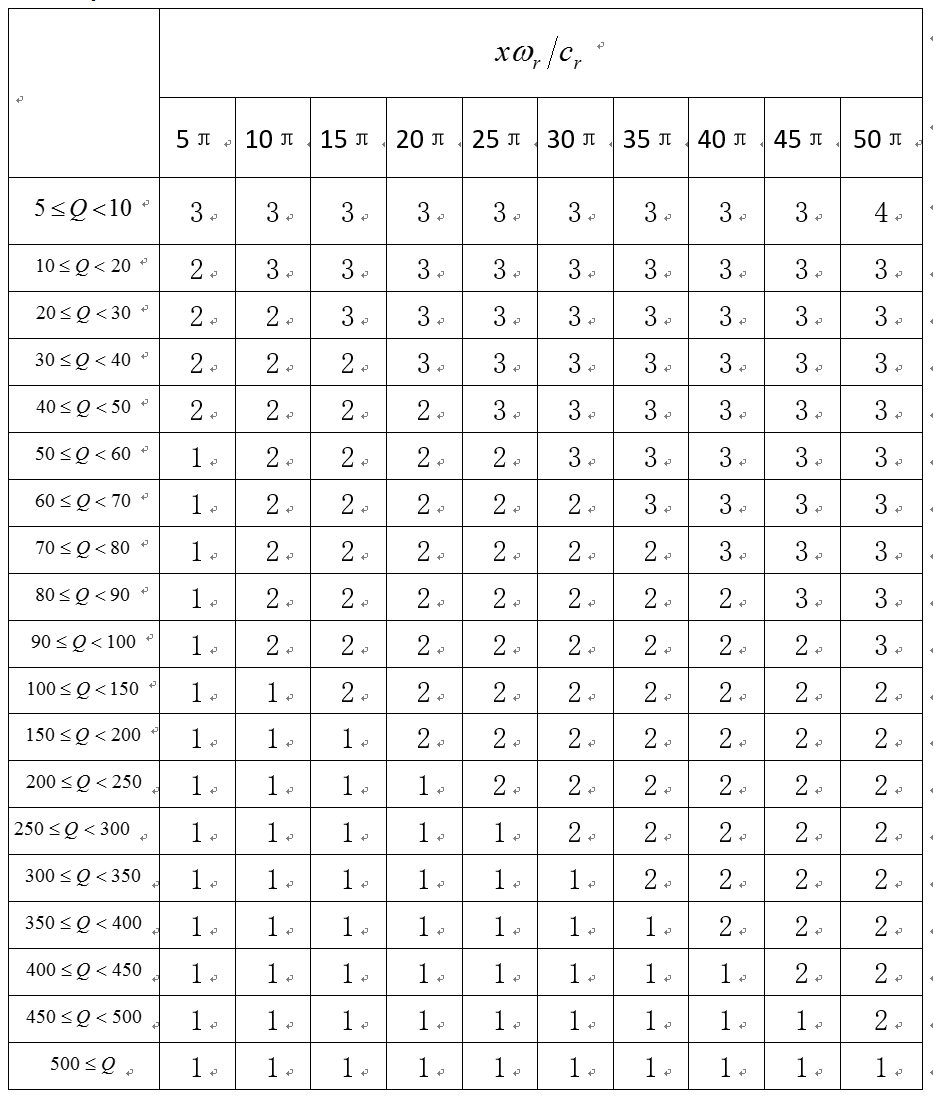
\includegraphics[width=5in]{figures/minimum_number_of_SLS_that_can_be_used_in_viscoelastic_simulation.png}
\caption{Table showing how you can select a value of N\_SLS smaller than 3, if and only if you know what you are doing.}
\label{fig:selectNSLS}
\end{figure}
%%


%------------------------------------------------------------------------------------------------%
\section*{Notes about \texttt{DATA/SOURCE} parameters}
%------------------------------------------------------------------------------------------------%


The \texttt{SOURCE} file located in the \texttt{DATA/} directory should be edited in the following way:
%
\begin{description}[font=\ttfamily]
\item[source\_surf] Set this flag to \texttt{.true.} to force the source to be located at the surface of the model, otherwise
the sol be placed inside the medium

\item[xs] source location $x$ in meters

\item[zs] source location $z$ in meters

\item[source\_type] Set this value equal to \texttt{1} for elastic forces or acoustic pressure,
set this to \texttt{2} for moment tensor sources.
For a plane wave including converted and reflected waves at the free surface, P wave = 1, S wave = 2, Rayleigh wave = 3;
for a plane wave without converted nor reflected waves at the free surface, i.e. the incident wave only, P wave = 4, S wave = 5.
(incident plane waves are turned on by parameter \texttt{initialfield} in \texttt{DATA/Par\_file}).

\item[time\_function\_type] Choose a source-time function: set this value to \texttt{1} to use a Ricker, i.e. the second derivative of a Gaussian,
\texttt{2} to use the first derivative of a Gaussian, \texttt{3} to use a Gaussian, \texttt{4} to use a Dirac or \texttt{5} to use a Heaviside source-time function.
Note that we use the standard definition of a Ricker, for a dominant frequency $f_0$:
$\mathrm{Ricker}(t) = (1 - 2 a t^2) e^{-a t^2}$, with $a = \pi^2 f_0^2$,
whose Fourier transform is thus:
$\frac{1}{2} \frac{\sqrt{\pi}\omega^2}{a^{3/2}}e^{-\frac{\omega^2}{4 a}}$
This gives the wavelet of Figure~\ref{fig:RickerWavelet}.
%%
\begin{figure}[htbp]
\centering
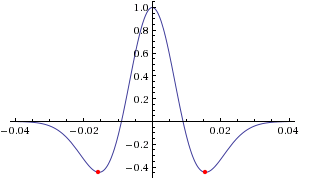
\includegraphics[width=3in]{figures/Ricker_wavelet.png}
\caption{We use the standard definition of a Ricker (i.e., second derivative of a Gaussian). Image taken from \url{http://subsurfwiki.org}.}
\label{fig:RickerWavelet}
\end{figure}
%%

\item[f0] Set this to the dominant frequency of the source.
For point-source simulations using a Heaviside source-time function (\texttt{time\_function\_type = 5}),
we recommend setting the source frequency parameter \texttt{f0}
equal to a high value, which corresponds to simulating a step source-time
function, i.e., a moment-rate function that is a delta function.

The \texttt{half duration} of a source is obtained by $1/\mathtt{f0}$.
If the code will use a Gaussian source-time function (\texttt{time\_function\_type = 3})
(i.e., a signal with a shape similar to a `smoothed triangle', as
explained in \citet{KoTr02a} and shown in Fig~\ref{fig:gauss.vs.triangle}), the
source-time function uses a half-width of \texttt{half duration}. We prefer
to run the solver with \texttt{half duration} set to zero and convolve
the resulting synthetic seismograms in post-processing after the run,
because this way it is easy to use a variety of source-time functions.
\citet{KoTr02a} determined
that the noise generated in the simulation by using a step source
time function may be safely filtered out afterward based upon a convolution
with the desired source time function and/or low-pass filtering. Use
the serial code \texttt{convolve\_source\_timefunction.f90} and the
script \texttt{convolve\_source\_timefunction.sh} for this purpose,
or alternatively use signal-processing software packages such as SAC \urlwithparentheses{www.llnl.gov/sac}.
Type
%
\begin{verbatim}
    make xconvolve_source_timefunction
\end{verbatim}
%
to compile the code and then set the parameter \texttt{hdur} in \texttt{convolve\_source\_timefunction.sh}
to the desired half-duration.
%%
\begin{figure}[htbp]
\centering
\includegraphics[width=3in]{figures/gauss_vs_triangle_mod.pdf}
\caption{Comparison of the shape of a triangle and the Gaussian function actually
used.}
\label{fig:gauss.vs.triangle}
\end{figure}
%%

\item[t0] For single sources, we recommend to set the time shift parameter \texttt{t0} equal to $0.0$.
The time shift parameter would simply apply
an overall time shift to the synthetics (according to the time shift of the first source), something that can be done
in the post-processing. This time shift parameter can be non-zero when using multiple sources.

\item[anglesource] angle of the source (for a force only); for a plane wave, this is the incidence angle. For moment tensor sources this parameter is unused.

\item[Mxx,Mzz,Mxz] Moment tensor components (valid only for moment tensor sources, \texttt{source\_type = 2}).
Note that the units for the components of a moment tensor source are different in SPECFEM2D and in SPECFEM3D:
%
\begin{description}
\item[SPECFEM3D:] in SPECFEM3D the moment tensor components are in dyne*cm
\item[SPECFEM2D:] in SPECFEM2D the moment tensor components are in N*m
\end{description}

To go from strike / dip / slip to CMTSOLUTION moment-tensor format using the classical formulas (of e.g. \cite{AkRi80} you can use these two small C programs from \texttt{SPECFEM3D\_GLOBE}:

\texttt{./utils/strike\_dip\_rake\_to\_CMTSOLUTION.c}

\texttt{./utils/CMTSOLUTION\_to\_AkiRichards.c}

but then it is another story to make a good 2D approximation of that, because in plain-strain P-SV what you get is the equivalent of a line source in the third direction (orthogonal to the plane) rather than a 3D point source
For more details on this see e.g. Section 7.3 "Two-dimensional point sources" of the book of \cite{Pil79}. That book being hard to find, we scanned the related pages in file\\
\texttt{discussion\_of\_2D\_sources\_and\_approximations\_from\_Pilant\_1979.pdf} in the same directory as this users manual.
Another very useful reference addressing that is \cite{HeVi88} and its recent extension \citep{LiHeClSu14}.

\item[factor] amplification factor

\end{description}

Note, the zero time of the simulation corresponds to the center of the triangle/Gaussian,
or the centroid time of the earthquake. The start time of the simulation
is $t=-1.2*\mathtt{half~duration} + \mathtt{t0}$ (the factor 1.2 is to make sure the moment
rate function is very close to zero when starting the simulation; Heaviside functions use a factor 2.0),
the half duration is obtained by $1/\mathtt{f0}$.
If you prefer, you can fix this start time by setting the parameter \texttt{USER\_T0} in the \texttt{constants.h} file
to a positive, non-zero value. The simulation in that case would start at a starting time equal to \texttt{-USER\_T0}.


%------------------------------------------------------------------------------------------------%
\section{How to run elastic wave simulations}
%------------------------------------------------------------------------------------------------%

For isotropic elastic materials, there are two options:
%
\begin{description}
\item[P-SV:]
To run a P-SV waves calculation propagating in the $x$-$z$ plane,
set \texttt{p\_sv = .true.} in the \texttt{Par\_file}.

\item[SH:]
To run a SH (membrane) waves calculation travelling in the $x$-$z$ plane with a
$y$-component of motion, set \texttt{p\_sv = .false.}

\end{description}
%
This feature is only implemented for elastic materials and sensitivity kernels
can be calculated (see \cite{TaLiTr07} for details on membrane
surface waves).

An optional useful Python script called \texttt{SEM\_save\_dir.py} is provided.
It allows one to automatically save all the parameters and results of a given simulation.
%------------------------------------------------------------------------------------------------%

%------------------------------------------------------------------------------------------------%
\section{How to run axisymmetric wave simulations}
\label{sec:axisym}
%------------------------------------------------------------------------------------------------%
Axisymmetric simulations are possible in SPECFEM2D. For these simulations the 2D domain simulated is physically the meridional 2D shape of an axisymmetric 3D domain.
We invite you to read our publication \citep{BoCrKoAs16} as an introduction.
To set the geometry as axisymmetric turn the flag \texttt{AXISYM} to \texttt{.true.} in the \texttt{Par\_file}:
\begin{verbatim}
   AXISYM                          = .true.
\end{verbatim}
The left border of the model becomes then a symmetry axis. The wavefield calculated is then physically a 3D wavefield obtained by revolution of a 2D wavefield
around its left border.
\\\\
Note about the source:\\
In axisymmetric geometry the whole model is symmetric with respect to this axis, including the source. Hence if the source is not on the axis it will physically
have a circular shape. This is still possible and relevant for some applications as non destructive testing but
is most of the time unwanted. This has to be kept in mind. In acoustic medium, as an explosion in a fluid is naturally axisymmetric, the wavefield generated has the
correct 3D shape. However, if the source is put in an elastic solid, its 3D radiation pattern will be axisymmetric.
\\\\
Getting started:\\
To get started a simple example is available in
\texttt{EXAMPLES/axisymmetric\_case\_AXISYM\_option}, we encourage you to read the \texttt{README} file you will find there.
This example contains an example of the use of \texttt{AXISYM} option plus a validation using the semi-analytical code OASES (\cite{Oases2004}).
In this example the domain studied is a water layer lying above a viscoelastic medium. The source is an explosion in the water and the domain is bounded with PMLs.
\\\\
Note about external meshers:\\
Using external meshers is possible in axisymmetric geometry. An example is available in \\ \texttt{EXAMPLES/paper\_axisymmetry\_example} with the mesher
Cubit/Trelis (\url{http://www.csimsoft.com/trelis}).
We invite you to check this example and read the previous chapter for more details. The only difference with plane-strain geometry is that SPECFEM2D needs an additional file defining
axial elements. The path to this file has to be given in the \texttt{Par\_file}:
\begin{verbatim}
   axial_elements_file             = /path/to/the/axial_elements_file
\end{verbatim}
The axial elements file has the following structure:
\begin{verbatim}
        48
         1          2       8456       8457
         2          2       8457       8458
         3          2       8458       8459
         4          2       8459       8460
       623          2        171        204
      1053          2        172       9512
      1054          2        172        173
      1055          2        173        174
      ...
\end{verbatim}
Which is similar to free surface files. Hence the first line contains the number of axial elements, then the other lines contain four columns:
element id, number of nodes describing an axial element (always 2), first node id, second node id.
Note that the axis elements must include the possible (up and/or down) PMLs elements in contact with the axis.
For simplicity we assume that the mesh elements that are in contact with the symmetry axis are in contact with it
by a full edge rather than by a single point, i.e. we exclude cases as that of Figure~\ref{fig:meshrestrictionontheaxis}.
This amounts to imposing that the leftmost layer of elements in the mesh be structured rather than non structured; The rest of the mesh can be non structured.
\begin{figure}
%\centerline{\includegraphics[width=0.38\linewidth]{FIGURES/case_that_we_exclude_for_axisymmetric_mesh.eps}}
\centerline{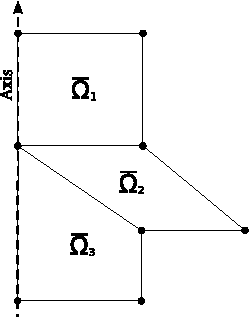
\includegraphics[width=0.38\linewidth]{figures/meshrestrictionontheaxis-eps-converted-to.pdf}}
\caption{\label{fig:meshrestrictionontheaxis} For simplicity we exclude cases in which the mesh elements that are in contact with the symmetry axis
are in contact with it by a single point instead of by a full edge, such as element $\bar{\Omega}_2$ here.
This amounts to imposing that the leftmost layer of elements in the mesh be structured rather than non structured; The rest of the mesh can be non structured.}
\end{figure}
\\\\
Note about the resolution:\\
In axisymmetry a different quadrature is used in the axial elements making the number of points per wavelength necessary a slightly
bigger ($\approx 25\%$) than in plane-strain.
\\\\
Note about a small remaining bug:\\
It has to be noted that a small bug is still hiding somewhere in the code. Indeed the output signals generated are correct in the
whole domain except in the element containing the source. This small bug has not been solved so far but not prevent to use the code.
\\\\
Note about a demo code to learn:\\
A simplistic demo code is available in \\ \texttt{utils/small\_SEM\_solver\_in\_Fortran\_without\_MPI\_to\_learn}.
This simple code is useful to learn how the spectral-element method works in both plane-strain and axisymmetric geometries.
Have a look to it if interested. Once in its directory, type \texttt{./make\_Fortran\_2D\_axisymmetric.csh} and then \texttt{./xspecfem2D}
to compile and run. The bug discussed above is not present in this small code.
%------------------------------------------------------------------------------------------------%

%------------------------------------------------------------------------------------------------%
\section{How to run anisotropic wave simulations}
%------------------------------------------------------------------------------------------------%

Following \cite{CaKoKo88}, we use the classical reduced Voigt notation to represent symmetric
tensors \citep{Hel94,Car07}:
%
\begin{quotation}
The constitutive relation of a heterogeneous anisotropic and elastic solid
is expressed by the generalized Hooke's law, which can be written as
%
\begin{equation*}
\sigma_{ij} = c_{ijkl} \varepsilon_{kl}, \qquad i, j, k = 1, \dots, 3,
\end{equation*}
%
where $t$ is the time, $\mathbf{x}$ is the position vector, $\sigma_{ij}(\mathbf{x}, t)$ and $\varepsilon_{ij}(\mathbf{x}, t)$ are the
Cartesian components of the stress and strain tensors respectively, and
$c_{ijkl}(\mathbf{x})$ are the components of a fourth-order tensor called the elasticites of
the medium. The Einstein convention for repeated indices is used.

To express the stress-strain relation for a transversely isotropic medium
we introduce a shortened matrix notation commonly used in the literature.
With this convention, pairs of subscripts concerning the elasticities are
replaced by a single number according to the following correspondence:
%
\begin{align*}
(11) \rightarrow 1, &&
(22) \rightarrow 2, &&
(33) \rightarrow 3, \\
(23) = (32) \rightarrow 4, &&
(31) = (13) \rightarrow 5, &&
(12) = (21) \rightarrow 6.
\end{align*}
\end{quotation}
%
Thus in the most general 2D case we have the following convention for the stress-strain relationship:
%
\begin{verbatim}
! implement anisotropy in 2D
sigma_xx = c11*dux_dx + c13*duz_dz + c15*(duz_dx + dux_dz)
sigma_zz = c13*dux_dx + c33*duz_dz + c35*(duz_dx + dux_dz)
sigma_xz = c15*dux_dx + c35*duz_dz + c55*(duz_dx + dux_dz)

! sigma_yy is not equal to zero in the plane strain formulation
! but is used only in post-processing if needed,
! to compute pressure for display or seismogram recording purposes
sigma_yy = c12*dux_dx + c23*duz_dz + c25*(duz_dx + dux_dz)
\end{verbatim}
%
where the notations are for instance \texttt{duz\_dx = d(Uz) / dx}.


%------------------------------------------------------------------------------------------------%
\section{How to run poroelastic wave simulations}
%------------------------------------------------------------------------------------------------%

Check the following new inputs in \texttt{Par\_file}:
%
\begin{description}[style=nextline, labelindent=1em, font=\normalfont]
\item[In section \textbf{"\# geometry of model and mesh description"}:]
\texttt{TURN\_VISCATTENUATION\_ON}, \texttt{Q0}, and \texttt{FREQ0} deal with viscous damping in a poroelastic medium.
\texttt{Q0} is the quality factor set at the central frequency \texttt{FREQ0}. For more details
see \cite{MoTr08}.

\item[In section \textbf{"\# time step parameters"}:]
\texttt{SIMULATION\_TYPE} defines the type of simulation
  \begin{enumerate}[label=(\arabic*)]
    \item forward simulation
    \item UNUSED (purposely, for compatibility with the numbering convention used in our 3D codes)
    \item adjoint method and kernels calculation
  \end{enumerate}

\item[In section \textbf{"\# source parameters"}:]
The code now support multiple sources.
\texttt{NSOURCE} is the number of sources.
Parameters of the sources are displayed in the file \texttt{SOURCE}, which must be
in the directory \texttt{DATA/}. The components of a moment tensor source must be given in N.m,
not in dyne.cm as in the \texttt{DATA/CMTSOLUTION} source file of the 3D version of the code.
%%%
\begin{figure}[htbp]
\centering
\includegraphics[width=5in]{figures/source_timing.pdf}
\caption{Example of timing for three sources. The center of the first source
triangle is defined to be time zero. Note that this is NOT in general
the hypocentral time, or the start time of the source (marked as \texttt{tstart}).
The time shift parameter \texttt{t0} in the \texttt{SOURCE} file
would be $t1(=0)$, $t2$, $t3$ in this case, and the half-duration parameter, \texttt{f0},
would be $\mathtt{hdur1}=1/\mathtt{f0}_1$, $\mathtt{hdur2}=1/\mathtt{f0}_2$,
$\mathtt{hdur3}=1/\mathtt{f0}_3$ for the sources 1, 2, 3 respectively.}
\label{fig:source_timing}
\end{figure}
%%%


\item[In section \textbf{"\# receiver line parameters for seismograms"}:]
\texttt{SAVE\_FORWARD} determines if the last frame of a forward simulation is saved (\texttt{.true.}) or not (\texttt{.false})

\item[In section \textbf{"\# define models...."}:]
There are three possible types of models:
  \begin{enumerate}[label=\ttfamily \Roman*:]
    \item (\texttt{model\_number 1 rho Vp Vs 0 0 QKappa Qmu 0 0 0 0 0 0}) or
    \item (\texttt{model\_number 2 rho c11 c13 c15 c33 c35 c55 c12 c23 c25 0 0 0}) or
    \item (\texttt{model\_number 3 rhos rhof phi c kxx kxz kzz Ks Kf Kfr etaf mufr Qmu}).
  \end{enumerate}

For isotropic elastic/acoustic material use \texttt{I} and set \texttt{Vs} to zero to make a given model acoustic, for anisotropic elastic use \texttt{II},
and for isotropic poroelastic material use \texttt{III}. The mesh can contain acoustic, elastic, and poroelastic models simultaneously.

For anisotropic elastic media the last three parameters, \texttt{c12 c23 c25}, are used only when the user asks the code to compute pressure for display
or seismogram recording purposes. Thus, if you do not know these parameters for your anisotropic material and/or if you do not plan to display or record pressure you
can ignore them and set them to zero. When pressure is used these three parameters are needed because the code needs to compute $\sigma_{yy}$,
which is not equal to zero in the plane strain formulation.

\begin{description}[font=\ttfamily, labelindent=1em, labelsep=1ex]
\item[rho\_s] = solid density
\item[rho\_f] = fluid density
\item[phi] = porosity
\item[tort] = tortuosity
\item[permxx] = xx component of permeability tensor
\item[permxz] = xz,zx components of permeability tensor
\item[permzz] = zz component of permeability tensor
\item[kappa\_s] = solid bulk modulus
\item[kappa\_f] = fluid bulk modulus
\item[kappa\_fr] = frame bulk modulus
\item[eta\_f] = fluid viscosity
\item[mu\_fr] = frame shear modulus
\item[Qmu] = shear quality factor
\end{description}

Note: for the poroelastic case, \texttt{mu\_s} is irrelevant.
For details on the poroelastic theory see \cite{MoTr08}.

\end{description}

\texttt{get\_poroelastic\_velocities.f90} allows to compute cpI, cpII, and cs function of
the source dominant frequency. Notice that for this calculation we use \texttt{permxx}
and the dominant frequency of the first source, f0(1). Caution if you use
several sources with different frequencies and if you consider anistropic
permeability.

%------------------------------------------------------------------------------------------------%
\section{Coupled simulations}
%------------------------------------------------------------------------------------------------%

The code supports acoustic/elastic, acoustic/poroelastic, elastic/poroelastic,
and acoustic, elastic/poroelastic simulations.
Elastic/poroelastic coupling supports anisotropy, but not attenuation for the
elastic material.


%------------------------------------------------------------------------------------------------%
\section{How to choose the time step}
%------------------------------------------------------------------------------------------------%

Three different explicit conditionally-stable time schemes can be used for elastic, acoustic (fluid) or coupled elastic/acoustic media:
the Newmark method, the low-dissipation and low-dispersion fourth-order six-stage Runge-Kutta method (LDDRK4-6) presented in \cite{BeBoBa06},
and the classical fourth-order four-stage Runge-Kutta (RK4) method.
Currently the last two methods are not implemented for poroelastic media.
According to \cite{DeSe10} and \cite{BeBoBa06}, with different degrees $N=NGLLX-1$ of the GLL basis functions the CFL bounds are given in the following tables.
Note that by default the SPECFEM solver uses $NGLLX = 5$ and thus a degree $N = 4$, which is thus the value you should use
in most cases in the following tables.
You can directly compare these values with the value given in sentence `Max stability for P wave velocity' in file
\texttt{output\_solver.txt} to see whether you set the correct $\Delta t$ in \texttt{Par\_file} or not.
For elastic simulation, the
CFL value given in \texttt{output\_solver.txt} does not consider the $V_p/V_s$ ratio, but the CFL limit slight decreases when $V_p/V_s$ increases.
In viscoelastic simulations the CFL limit does not change compared to the elastic case because we use a rational approximation of a constant quality factor Q, which has no attenuation effect on zero-frequency waves.
Additionally, if you use C-PML absorbing layers in your simulations, which are implemented for the Newmark and LDDRK4-6 techniques but not for the classical RK4), the CFL upper limit decreases to approximately 95\% of the limit without absorbing layers in the case of Newmark and to 85\% in the case of LDDRK4-6.
\begin{table}[htbp]
\caption{CFL upper bound for an acoustic (fluid) simulation.}
% title of Table
\centering
% used for centering table
\begin{tabular}{c c c c}
% centered columns (4 columns)
\hline\hline
%inserts double horizontal lines
Degree $N$ & Newmark & LDDRK4-6 & RK4 \\ [0.5ex]
% inserts table
%heading
\hline
% inserts single horizontal line
1 & 0.709 & 1.349 & 1.003 \\
2 & 0.577 & 1.098 & 0.816 \\
3 & 0.593 & 1.129 & 0.839 \\
\red{4} & \red{0.604} & \red{1.150} & \red{0.854} \\
5 & 0.608 & 1.157 & 0.860 \\
6 & 0.608 & 1.157 & 0.860 \\
7 & 0.608 & 1.157 & 0.860 \\
8 & 0.607 & 1.155 & 0.858 \\
9 & 0.607 & 1.155 & 0.858 \\
10 & 0.607 & 1.155 & 0.858 \\ [1ex]
% [1ex] adds vertical space
\hline
%inserts single line
\end{tabular}
\label{table:CFLacoustic}
% is used to refer this table in the text
\end{table}
%
\begin{table}[htbp]
\caption{CFL upper bound for an elastic simulation with $V_p/V_s = \sqrt{2}$.}
% title of Table
\centering
% used for centering table
\begin{tabular}{c c c c}
% centered columns (4 columns)
\hline\hline
%inserts double horizontal lines
Degree $N$ & Newmark & LDDRK4-6 & RK4 \\ [0.5ex]
% inserts table
%heading
\hline
% inserts single horizontal line
1 & 0.816 & 1.553 & 1.154 \\
2 & 0.666 & 1.268 & 0.942 \\
3 & 0.684 & 1.302 & 0.967 \\
\red{4} & \red{0.697} & \red{1.327} & \red{0.986} \\
5 & 0.700 & 1.332 & 0.990 \\
6 & 0.700 & 1.332 & 0.990 \\
7 & 0.700 & 1.332 & 0.990 \\
8 & 0.699 & 1.330 & 0.989 \\
9 & 0.698 & 1.328 & 0.987 \\
10 & 0.698 & 1.328 & 0.987 \\ [1ex]
% [1ex] adds vertical space
\hline
%inserts single line
\end{tabular}
\label{table:CFLelastic}
% is used to refer this table in the text
\end{table}

%------------------------------------------------------------------------------------------------%
\section{How to set plane waves as initial conditions}
%------------------------------------------------------------------------------------------------%

To simulate propagation of incoming plane waves in the simulation domain, initial conditions based on analytical formulae of plane waves in homogeneous model need to be set. No additional body or boundary forces are required. To set up this scenario:
%
\begin{description}
\item{\verb+Par_file+:}
  \begin{itemize}
  \item switch on \verb+initialfield = .true. +
  \item at this point setting \verb+add_bielak_condition+ does not seem to help with absorbing boundaries, therefore, it should be turned off.
  \end{itemize}
\item{\verb+SOURCE+:}
  \begin{itemize}
  \item \verb+zs+ has to be the same as the height of the simulation domain defined in \verb+interfacesfile+.
  \item \verb+xs+ is the $x$-coordinate of the intersection of the initial plane wave front with the free surface.
  \item \verb+source_type+ = 1 for a plane P wave, 2 for a plane SV wave, 3 for a Rayleigh wave.
  \item \verb+angleforce+ can be negative to indicate a plane wave incident from the right (instead of the left)
  \end{itemize}
\end{description}

%------------------------------------------------------------------------------------------------%
\section{Note on the viscoelastic model used}
%------------------------------------------------------------------------------------------------%

\noindent
The model used is a constant $Q$, thus with no dependence on frequency ($Q(f)$ = constant).
See e.g. \cite{BlKoChLoXi16}. \\

\noindent
However in practice for technical reasons it is approximated based on the sum of different Generalized Zener body mechanisms
and thus the code outputs the band in which the approximation is very good, outside of that range it can be less accurate.
The logarithmic center of that frequency band is the \texttt{f0} parameter defined (in Hz) in input file \texttt{DATA/SOURCE}.

%------------------------------------------------------------------------------------------------%
\section{Note on viscoelasticity in the 2D plane strain approximation}
%------------------------------------------------------------------------------------------------%

\noindent
In 2D plane strain, one spatial dimension is much greater than the others (see for example: \url{http://www.engineering.ucsb.edu/~hpscicom/projects/stress/introge.pdf})
and thus $\kappa = \lambda + \mu$ in 2D plane strain (instead of $\kappa = \lambda + \frac{2}{3} \mu$ in 3D).
See for example \cite{CaKoKo88b} equation (A9), and equation 6 in \url{http://cherrypit.princeton.edu/papers/paper-99.pdf}. \\

\noindent
In 2D axisymmetric I think the 2/3 coefficient is OK, but it would be worth doublechecking.

